\section{Description and methodology}


The whole exercise was done in small increments. We started by learning how to control the LEDs. Then we made registering button presses work, followed by altering the LEDs on a button press. Finally we combined everything together with an interrupt routine. We will now look more closely on each step.

\subsection{Overall hardware setup}

All jumper settings were checked and done as described in the exercise description. We connected the LEDs with an 8-pin flat cable to the GPIO pins 0-7, which are mapped to PIOB pins 0-7. A second 8-pin flat cable connected buttons 0-7 to GPIO pins 16-23, which are mapped to PIOC pins 0-7.

\subsection{Controlling the LEDs}

With our setup the 8 LEDs can be controlled through PIO port B pins 0 - 7. We started by enabling these pins on the IO-controller. This is done by writing 0b11111111 to the address for PIOB + offset for the enable register (called PIO\_PER). Next we enabled output on the pins by writing 0b11111111 to the address for PIOB + offset for the enable output register (called PIO\_OER). Which LEDs are actually turned on can be controlled by writing to the register with offset PIO\_SODR, and turned off by writing to the register with offset PIO\_CODR, together with an 8-bit bitmask corresponding to LED 0-7.

\subsection{Buttons}

The buttons SW0-7 were in our case connected to GPIO pins 16-23, which in turn are connected to PIO port C pins 0-7. These are enabled by writing to PIO port Cs address plus the offset PIO\_PER. Since these are reading changes in value, we also need to enable the pull-up resistors by writing to the corresponding enable register. The status of these buttons can be read by copying from address (reading register) PIO\_C + PIO\_PDSR, where the lower-most byte corresponds to the status of the 8 buttons.

\subsection{Interrupts}

The AVR32 supports interrupt driven IO. To enable interrupts on our buttons several things must be taken care of. First we need to tell the IO-controller to enable interrupts on the buttons. This is done by writing to register with address PIOC + offset PIO\_IER. Next the interrupt controller needs to get an address (14 bits) in the register corresponding to interrupts from PIO\_C on line 0. The code at this address is the interrupt routine code that will be called. This address is called the autovector. The full address for the code called however, is the result of the variable EVBA + the autovector. In this exercise we can set the EVBA to 0 and just pass the address for where our interrupt routine resides, which helps simplify. Lastly we must enable interrupts for the whole system by setting the GM bit, done by the instruction \texttt{csrf 16}.

\subsection{Main program}
%\pagebreak
\begin{figure}[here]
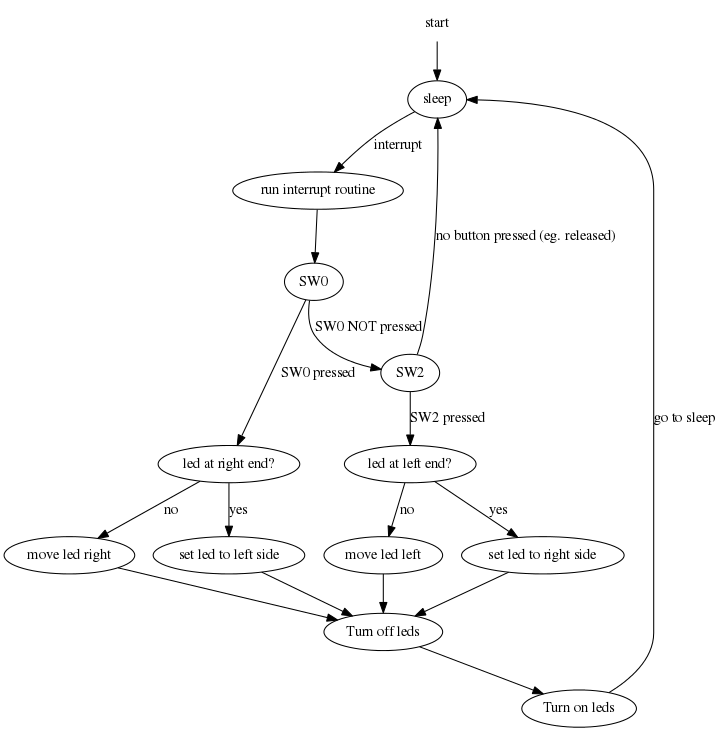
\includegraphics[width=0.9\textwidth]{img/graph.png}
\caption{Flowchart showing the flow of the main program loop and the interrupt routine. Notice the button precedence.}
\label{fig:mainflow}
\end{figure}

\begin{table}
 \centering
 \begin{tabular}{| c | l |}
    \hline
    \textsc{CPU Register} & \textsc{Contains} \\ \hline
    \texttt{r0} &       Address for PIO port B \texttt{PIOB}. \\
    \texttt{r1} &       Address for PIO port C \texttt{PIOC}. \\
    \texttt{r2} &       Address for interrupt controller \texttt{INTC}. \\
    \texttt{r7} &	Bitmask for enabled LEDs (lower most 8 bits) \\
    \hline
 \end{tabular}
 \caption{CPU registers used}
 \label{table:cpuregs}
\end{table}

The main program is a loop structured as the flowchart of Figure \ref{fig:mainflow}. We start off however by loading the addresses of PIOB, PIOC and the IO controller into registers r0, r1 and r2, respectively (not shown in figure). We then continue to set up the different io controllers and cpu as described in the sections above. The autovector is set to the address of the \texttt{handle\_interrupt} routine. The routine first determines if one of our predetermined buttons caused the interrupt, then figures out which one of these buttons is pressed right now, if any. If the correct button is pressed during the interrupt, the program then does a logical right or left shift of the LED lights, according to the button that was pressed. If the result after the logical shift is too big, or too small, the LEDs are reset to light up on the other end. E.g. if the value of the enabled LEDs is 0 after a logical right shift, it means that we should reset the light to show up on the other side. This works similarly for the left to right button, where we check if the value is bigger than the 8 lower bits. We then clear all the glowing LEDs and enable the row with the new bitmask, \texttt{rete} (return from interrupt) and go to sleep again. An overview of CPU registers in particular use is given in Table \ref{table:cpuregs}.


